\documentclass[letterpaper]{article}
\usepackage{aaai24}
\usepackage{times}
\usepackage{helvet}
\usepackage{courier}
\usepackage{graphicx}
\usepackage{amsmath,amssymb}
\usepackage{booktabs}
\usepackage{listings}
\usepackage{natbib}
\usepackage[hyphens]{url}
\usepackage{caption}
\urlstyle{rm}
\def\UrlFont{\rm}
\setlength{\pdfpagewidth}{8.5in}
\setlength{\pdfpageheight}{11in}
\pdfinfo{/TemplateVersion (2024.1)}
\nocopyright
\frenchspacing
\lstset{language=Python,basicstyle=\ttfamily\footnotesize,breaklines=true,columns=fullflexible,keepspaces=true,showstringspaces=false}
\title{Optimization and Regularization in EfficientNetV2-S\protect\\for Dog Breed Identification}
\author{JI QIANKUN}
\affiliations{Nanyang Technological University\\AI6103 Deep Learning \& Applications}
\begin{document}
\maketitle
\begin{abstract}
Eight experiments totaling 1,545 epochs examine optimization and regularization
in a randomly initialized EfficientNetV2-S for 120-class dog breed recognition.
A 15-epoch sweep selects learning rate 0.05 by final training cross-entropy (CE).
Extending training to 300 epochs produces nearly perfect training accuracy
without comparable validation performance: cosine scheduling improves training
fit but leaves substantial overfitting. Weight decay $5\times10^{-4}$ lowers
final validation CE, and Mixup with $\alpha=0.2$ raises validation accuracy from
31.2459\% to 37.3777\%. One evaluation of the frozen epoch-300 Mixup model gives
38.0704\% accuracy on 1,534 test images. Experimental curves use the original
records; the Beta density is analytic. Results concern one seed and the supplied
data splits.
\end{abstract}

\section{2. Data Preprocessing and Experimental Design}
The supplied Dog Breed dataset contains 10,222 images: 7,155 training, 1,533
validation and 1,534 test images, spanning 120 breeds. We preserve the prescribed
splits and resize every image to $100\times100$ pixels. RGB channel statistics use
\emph{training images only}, after PIL bilinear resizing and conversion to $[0,1]$.
For channel $c$, $\mu_c=N^{-1}\sum_i x_{ic}$ and
$\sigma_c=\sqrt{N^{-1}\sum_i(x_{ic}-\mu_c)^2}$ over all resized training pixels;
normalization is $\hat x_c=(x_c-\mu_c)/\sigma_c$.
Table~\ref{tab:norm} gives the retained values. An independent float64
recomputation agrees within $6.90\times10^{-8}$; the original values are preserved
across experiments rather than recomputed from validation or test images.

\begin{table}[h]
\centering
\begin{tabular}{lrrr}\toprule
 & R & G & B\\\midrule
Mean & 0.477183402 & 0.452763587 & 0.392786026\\
Std. & 0.253416061 & 0.247967348 & 0.252266765\\\bottomrule
\end{tabular}
\normalsize
\caption{Training-only RGB population moments used in every experiment.}
\label{tab:norm}
\end{table}

The following code reproduces the actual preprocessing order. Training uses a
horizontal flip with probability 0.5, then 12 pixels of zero padding on every
side and a random $100\times100$ crop. Validation and test use deterministic
resizing, tensor conversion and the same training-derived normalization.
\begin{figure*}[t]
\centering
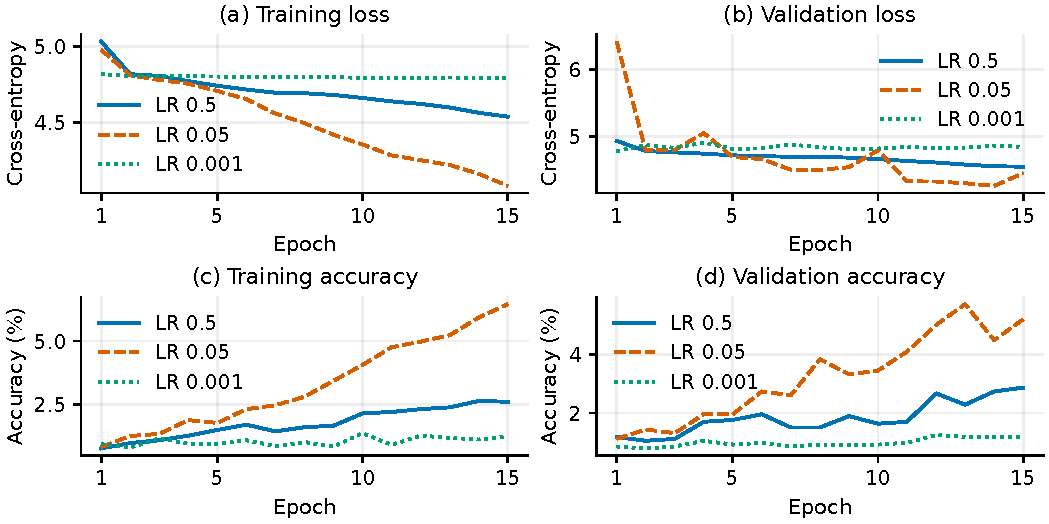
\includegraphics[width=\textwidth]{figures/section3_lr.pdf}
\caption{Section 3: every recorded epoch of the 15-epoch LR sweep. Lower CE is better;
accuracy is shown in percent. All runs use the same augmentation, initialization
seed and batch size, with no schedule or weight decay. LR 0.05 leads all four
\emph{final} metrics; the selection rule uses final training CE only.}
\label{fig:lr}
\end{figure*}

\noindent\begin{minipage}{\columnwidth}
\begin{lstlisting}
from torchvision import transforms as T

mean = (0.47718340158462524,
        0.4527635872364044,
        0.39278602600097656)
std = (0.2534160614013672,
       0.24796734750270844,
       0.2522667646408081)

train_tf = T.Compose([
    T.Resize((100, 100)),
    T.RandomHorizontalFlip(p=0.5),
    T.RandomCrop(100, padding=12, fill=0,
                 padding_mode="constant"),
    T.ToTensor(), T.Normalize(mean, std)])
eval_tf = T.Compose([
    T.Resize((100, 100)),
    T.ToTensor(), T.Normalize(mean, std)])
\end{lstlisting}
\end{minipage}

The training-only moment calculation uses the following accumulation, with
\texttt{loader} containing only resized, tensor-converted training images
(batch size 64, no shuffle or augmentation):
\begin{lstlisting}
sums = torch.zeros(3, dtype=torch.float64)
squares = torch.zeros(3, dtype=torch.float64)
n = 0
dims = (0, 2, 3)
for images, _ in loader:
    images = images.double()
    sums += images.sum(dims)
    squares += images.square().sum(dims)
    n += (images.shape[0] * images.shape[2]
          * images.shape[3])
mean = sums / n
std = (squares / n - mean.square())
std = std.clamp_min(0).sqrt()
\end{lstlisting}
This recomputation checks the retained normalization constants above; it does
not replace them for the completed experiments.

We use torchvision EfficientNetV2-S~\cite{tan2021efficientnetv2} with
\texttt{weights=None}, replacing the classifier with 120 outputs. Every experiment
starts from scratch and uses SGD, momentum 0.9, batch size 128, seed 6103 and
zero DataLoader workers. No pretrained weights or adaptive optimizer are used.
Each epoch aggregates all 56 training batches, including the final incomplete
batch, by sample count. Training CE and accuracy describe the augmented batches
encountered while the parameters are changing. They are accumulated in training
mode, rather than recomputed with the final epoch model on clean training images.
Validation instead evaluates that epoch's model on deterministic, unaugmented
inputs in evaluation mode. Reported losses are classification CE and exclude
the weight penalty. The plotted train--validation gap therefore combines
differences in generalization, input augmentation and model mode; it is a
descriptive diagnostic, not an isolated estimate of any one of these effects.

All runs used the recorded NVIDIA A40 environment with Python 3.12.15,
PyTorch 2.6.0+cu124 and torchvision 0.21.0+cu124 on NTU TC2 through SLURM.
Deterministic settings and seed were held fixed. This is a single-seed controlled
study, not an estimate of variation across seeds or devices. Integrity checks
identified 10 cross-split byte-identical image pairs: four train--validation,
five train--test and one validation--test. The supplied splits were retained;
this overlap limits statistical independence of the reported evaluation.
Only validation data informed downstream hyperparameter selection. Test-file
integrity checks did not calculate performance; test inference occurred only
after all experiments and final model freezing.



\section{3. Learning Rate}
We compare learning rates $0.5$, $0.05$ and $0.001$ for 15 epochs, without weight
decay or scheduling. Table~\ref{tab:lr} reports the final values and
Figure~\ref{fig:lr} shows all four trajectories.

\begin{table}[t]
\centering\small
\begin{tabular}{lrrrr}\toprule
LR & Train CE & Train acc. & Val. CE & Val. acc.\\\midrule
0.5 & 4.5366 & 2.5996 & 4.5576 & 2.8702 \\
0.05 & 4.0806 & 6.4570 & 4.4615 & 5.2185 \\
0.001 & 4.7907 & 1.2299 & 4.8513 & 1.1742 \\
\bottomrule\end{tabular}
\normalsize
\caption{Section 3 final metrics at epoch 15. Accuracies are percentages.}
\label{tab:lr}
\end{table}

\begin{figure*}[t]
\centering
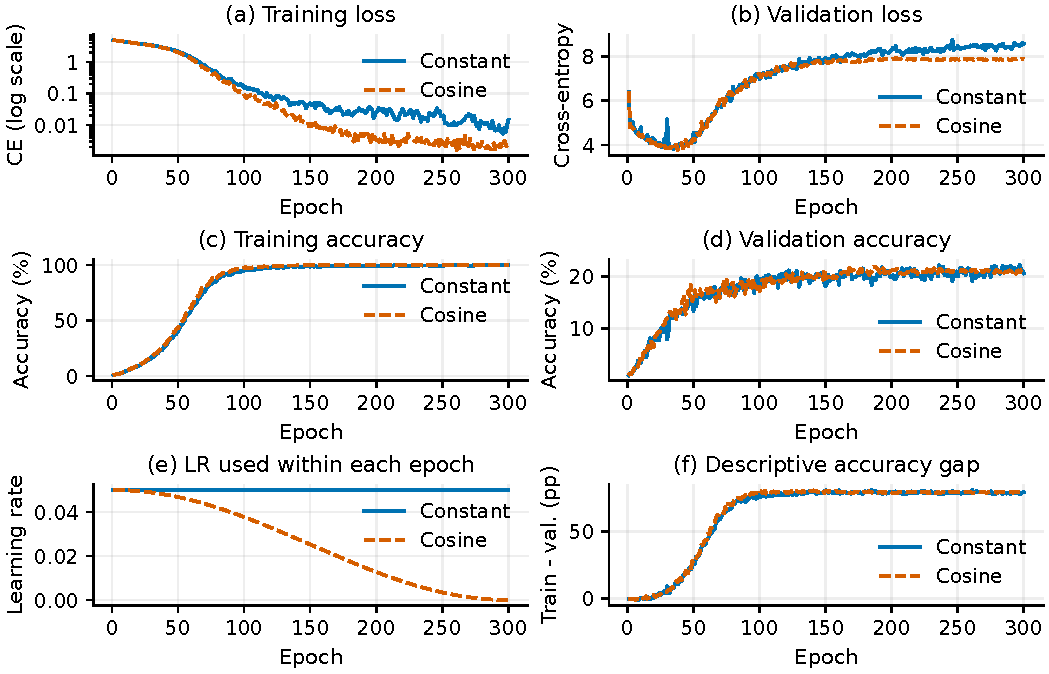
\includegraphics[width=\textwidth]{figures/section4_schedule.pdf}
\caption{Section 4: constant LR versus cosine, both starting at 0.05 with no weight
decay. Training CE uses a logarithmic axis so late optimization remains visible.
Panels (e)--(f) show the recorded within-epoch LR and descriptive accuracy gap.
Near-perfect training fit coexists with large validation CE in both conditions.}
\label{fig:schedule}
\end{figure*}

LR 0.05 has the lowest final training CE (4.0806) and highest training accuracy
(6.4570\%). It also has the lowest final validation CE (4.4615) and highest
validation accuracy (5.2185\%).

We select \textbf{0.05 strictly by final training loss}; agreement
with validation rankings does not change that rule. Its best validation
accuracy is 5.7404\% at epoch 13, illustrating that final and best-epoch
measurements are different quantities.

For LR 0.001, training CE (4.7907) is near the uniform-prediction loss
($\log120\simeq4.7875$), with 1.1742\% validation accuracy. It may have made
insufficient progress within 15 epochs; we did not test longer training. LR 0.5 fits better than 0.001 but worse than 0.05.
Its finite, gradually declining loss supports a limitation in optimization
efficiency rather than a claim of numerical divergence. Larger updates may
impede fitting, but curvature and update directions were not measured.
LR 0.05 also starts with validation CE 6.4095 and follows a non-monotonic
validation trajectory. Its winning endpoint therefore establishes the choice
for this seed and budget, not uniformly stable training or a universal optimum.


\section{4. Learning Rate Schedule}
Cosine annealing uses larger learning rates early in training and reduces them
smoothly for smaller late updates~\cite{loshchilov2017sgdr}. In this experiment,
one half-cosine covers all 300 epochs without a restart:
\begin{equation}
\eta_t=\frac{\eta_0}{2}\left(1+\cos\frac{\pi t}{T}\right),
\qquad\eta_0=0.05,\quad T=300.
\label{eq:cosine}
\end{equation}
Epoch $e$ uses $\eta_{e-1}$; the scheduler steps afterward and reaches zero
only after epoch 300. Midpoint LR is 0.025; all other settings remain fixed,
with no decay or restarts.

\begin{table}[t]
\centering\small
\begin{tabular}{lrrrr}\toprule
Schedule & Train CE & Train acc. & Val. CE & Val. acc.\\\midrule
Constant & 0.0143 & 99.6925 & 8.5748 & 20.6784 \\
Cosine & 0.0019 & 99.9720 & 7.8742 & 21.0698 \\
\bottomrule\end{tabular}
\normalsize
\caption{Section 4 final metrics at epoch 300; accuracies in percent.}
\label{tab:schedule}
\end{table}

\begin{figure*}[t]
\centering
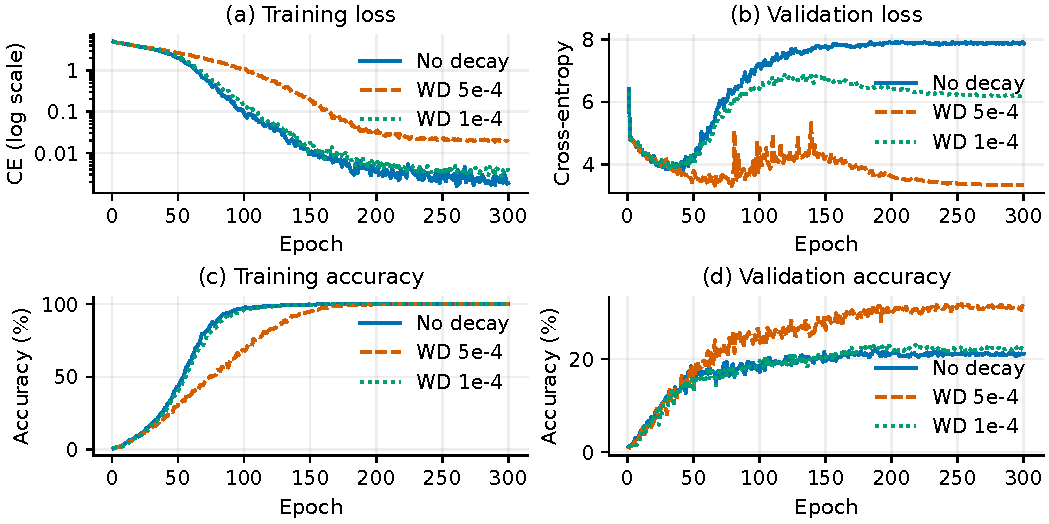
\includegraphics[width=\textwidth]{figures/section5_decay.pdf}
\caption{Section 5: the no-decay cosine baseline and both prescribed weight decays.
Training CE uses a log axis; validation CE and accuracies use linear axes.
All three use LR 0.05 and the same cosine schedule. Stronger decay substantially
improves validation behavior while the training accuracy remains near 100\%.}
\label{fig:decay}
\end{figure*}

Cosine reduces final training CE from 0.0143 to 0.0019 and raises training
accuracy from 99.6925\% to 99.9720\%. Validation accuracy improves only 0.3914
percentage points (pp), from 20.6784\% to 21.0698\%, while CE falls from 8.5748
to 7.8742. Cosine improves training fit but does not resolve overfitting
(Figure~\ref{fig:schedule}).

Validation CE is lowest at epoch 35 (3.8253, constant) and epoch 38 (3.7693,
cosine). Afterwards, training CE falls while validation CE rises, indicating
overfitting. CE depends on true-class probability, unlike top-1 accuracy;
increasingly confident errors may explain the CE rise, but confidence and
calibration were not measured.
The choice of summary also matters: constant LR reaches the higher \emph{best}
validation accuracy, 22.2440\% versus 21.9178\%, despite cosine's better final
accuracy. We report the required 300-epoch endpoints and retain the original
checkpoints rather than retrospectively introducing early stopping.


\section{5. Weight Decay}
For data loss $\mathcal L(w)$, adding a quadratic penalty gives
\begin{equation}
\mathcal L'(w)=\mathcal L(w)+\frac{\lambda}{2}\|w\|_2^2.
\end{equation}
Plain gradient descent then has the shrinkage interpretation
\begin{equation}
w_{t+1}=(1-\eta_t\lambda)w_t-\eta_t\nabla\mathcal L(w_t).
\end{equation}
We use coupled weight decay: SGD adds $\lambda w_t$ to the gradient before
momentum (0.9). Equation (3) explains shrinkage, not the full momentum update.
Reported CE excludes the penalty, so all settings use the same classification
loss; these curves do not show the penalized objective. The proposed mechanisms
depend on the optimizer and architecture and were not measured
here~\cite{zhang2019three}.

\begin{table}[t]
\centering\small
\begin{tabular}{lrrrr}\toprule
$\lambda$ & Train CE & Train acc. & Val. CE & Val. acc.\\\midrule
0 & 0.0019 & 99.9720 & 7.8742 & 21.0698 \\
$5\times10^{-4}$ & 0.0190 & 99.9581 & 3.3319 & 31.2459 \\
$10^{-4}$ & 0.0044 & 99.9441 & 6.1930 & 22.1135 \\
\bottomrule\end{tabular}
\normalsize
\caption{Epoch-300 weight-decay comparison with cosine; accuracies in percent.
The zero-decay row is the Section 4 cosine baseline.}
\label{tab:decay}
\end{table}

\begin{figure*}[t]
\centering
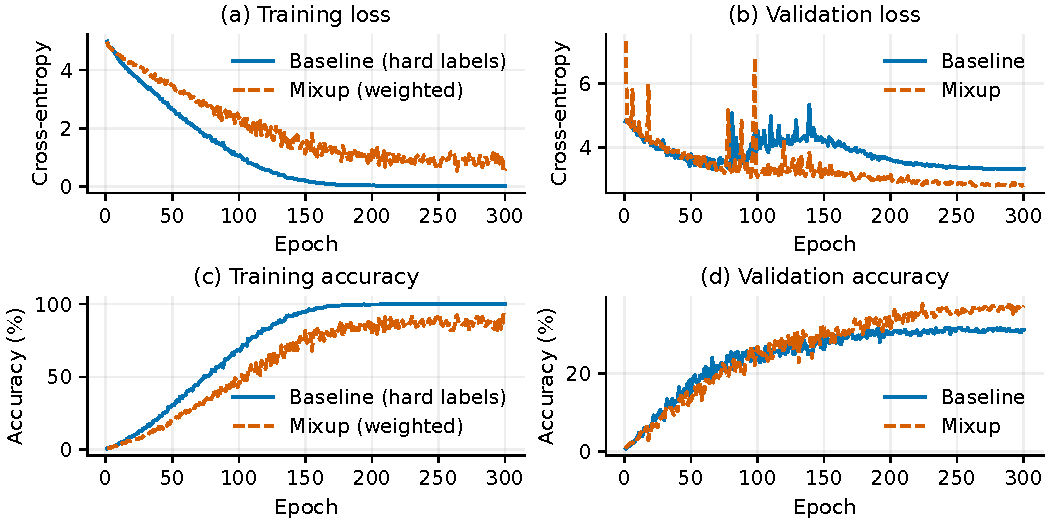
\includegraphics[width=\textwidth]{figures/section6_mixup.pdf}
\caption{Section 6: Mixup versus the verified $5\times10^{-4}$ cosine baseline.
Training CE and accuracy have mixed-label versus hard-label meanings, explicitly
marked in the legends; their vertical difference is not a like-for-like fitting
gap. Validation metrics share the same ordinary definitions and clean inputs.}
\label{fig:mixup}
\end{figure*}

With LR 0.05 and cosine fixed, decay $5\times10^{-4}$ achieves 31.2459\%
validation accuracy and CE 3.3319, outperforming weaker and zero decay
(Table~\ref{tab:decay}). It gains 10.1761 pp over no decay and limits late
validation-CE growth (Figure~\ref{fig:decay}).

All settings retain training accuracy above 99.94\%. Increasing decay from
$10^{-4}$ to $5\times10^{-4}$ raises training CE (0.0044 to 0.0190) but slightly
raises training accuracy, so the metrics show no simple trade-off. Weight norms
were not measured, so the mechanism remains uncertain. The stronger decay limits
late validation-CE growth and becomes our non-Mixup baseline
(Figure~\ref{fig:decay}).


\section{6. Data Augmentation with Mixup}
\subsection{Baseline Selection and Mixing Rule}
We select the baseline by final (epoch-300) validation CE across four verified
runs: constant (\texttt{sec4\_constant}, 8.5748), cosine
(\texttt{sec4\_cosine}, 7.8742), decay $5\times10^{-4}$
(\texttt{sec5\_wd5e-4}, 3.3319), and decay $10^{-4}$
(\texttt{sec5\_wd1e-4}, 6.1930). Ties follow this order; test data do not affect
selection. Mixup uses the winning decay ($5\times10^{-4}$) with LR 0.05, cosine,
the same seed and preprocessing, and trains from scratch for 300 epochs.

Mixup draws $\lambda\sim\operatorname{Beta}(\alpha,\alpha)$ with
$\alpha=0.2$~\cite{zhang2018mixup}. For a randomly permuted batch pairing,
\begin{align}
\widetilde x_i&=\lambda x_i+(1-\lambda)x_{\pi(i)},\\
\widetilde y_i&=\lambda y_i+(1-\lambda)y_{\pi(i)}.
\end{align}
The implementation draws one coefficient per batch and an independent random
permutation; it minimizes
\begin{equation}
\widetilde{\mathcal L}=\lambda\,\mathrm{CE}(f(\widetilde x_i),y_i)
 +(1-\lambda)\,\mathrm{CE}(f(\widetilde x_i),y_{\pi(i)}).
\end{equation}
This equals CE with the convex combination of one-hot targets, without
requiring explicit soft-label tensors. Images are mixed after the original
training augmentations and normalization. The saved RNG states preserve mixing
and permutation provenance. Validation images and labels are never mixed.

\begin{figure}[t]
\centering
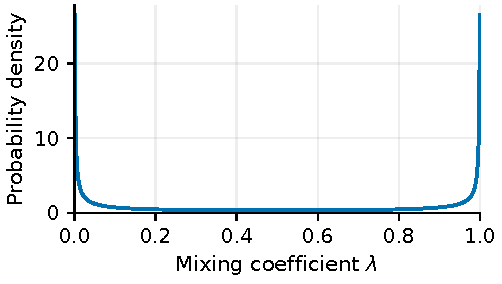
\includegraphics[width=\columnwidth]{figures/beta_02.pdf}
\caption{Analytic Beta$(0.2,0.2)$ PDF. Endpoints are excluded because their density
is unbounded. This curve is a mathematical function, not an experimental estimate.}
\label{fig:beta}
\end{figure}

\subsection{Distribution and Metric Interpretation}
The associated probability density is
\begin{equation}
p(\lambda)=\frac{\lambda^{-0.8}(1-\lambda)^{-0.8}}{B(0.2,0.2)},
\quad 0<\lambda<1.
\end{equation}
The Beta$(0.2,0.2)$ density is symmetric and U-shaped, favoring $\lambda$ near
0 or 1. Its endpoint densities diverge, although total probability is one.
Figure~\ref{fig:beta} plots the analytic density on $[0.001,0.999]$.


Training accuracy is the sample-weighted average of
$\lambda\mathbf1[\hat y=y_i]+(1-\lambda)\mathbf1[\hat y=y_{\pi(i)}]$.
This weighted agreement and mixed-target training CE differ from the baseline's
hard-label quantities. We therefore assess regularization mainly through the
common clean-validation CE and top-1 accuracy, not by treating the training
metrics as interchangeable.

\begin{table}[t]
\centering\small
\begin{tabular}{lrrrr}\toprule
Condition & Train CE & Train acc. & Val. CE & Val. acc.\\\midrule
No Mixup & 0.0190 & 99.9581 & 3.3319 & 31.2459 \\
Mixup & 0.6054 & 91.7724 & 2.8332 & 37.3777 \\
\bottomrule\end{tabular}
\normalsize
\caption{Section 6 final metrics at epoch 300. Accuracies in percent; Mixup
training metrics use the weighted definitions above.}
\label{tab:mixup}
\end{table}

\subsection{Observed Augmentation Effects}
Mixup raises final validation accuracy from 31.2459\% to 37.3777\%
(+6.1318 pp) and lowers CE from 3.3319 to 2.8332. Its training CE (0.6054) and
weighted accuracy (91.7724\%) use mixed targets and cannot be directly compared
with baseline training metrics (Table~\ref{tab:mixup}). For different paired
labels, a single prediction's weighted agreement is at most
$\max(\lambda,1-\lambda)$; the lower score does not show a loss of
clean-training accuracy.

Figure~\ref{fig:mixup} shows early validation fluctuations and better late
performance with Mixup. Training on mixed inputs and labels may improve
generalization by encouraging simpler behavior between
examples~\cite{zhang2018mixup}, but decision-boundary smoothness and robustness
were not measured. This supports Mixup for our baseline, not universal
superiority or optimal settings.

\begin{samepage}
The best Mixup validation accuracy is 37.8343\% at epoch 224, and its minimum
validation CE is 2.8082 at epoch 264. Neither checkpoint replaces the fixed
epoch-300 final model. Both final CE and final accuracy are reported because
minimizing CE need not maximize accuracy.\par
\end{samepage}

\subsection{Frozen Hold-out Evaluation}
The single final evaluation used the frozen epoch-300
\texttt{sec6\_mixup} checkpoint after the full experiment sequence. The freeze
manifest, evaluation claim, result and SLURM stdout identify the same checkpoint
(SHA256 beginning \texttt{787588449955}); the full hash and five original
evidence hashes are retained with the experiment records. The test did not
select a model or replace the frozen checkpoint.

TC2 Job 42825 tested the frozen model on 1,534 images using deterministic
preprocessing, training-derived normalization, and evaluation/inference mode.
Test accuracy was \textbf{38.0704\%} (\textbf{584 correct}, inferred rather than
logged), and CE was \textbf{2.7708}. The 0.6927 pp test--validation gap does not
prove model improvement because the splits differ. No test-based selection or
rerun occurred. The test-time selection flag was false; five evidence hashes
match the TC2 receipt, and stderr was empty.

These estimates apply to the supplied split and this fixed model. One seed,
finite test size and the documented duplicate-image overlap limit their
interpretation as performance on an independent population of future images.
No additional experiments or test-informed model changes are claimed.

\label{bodyend}
\typeout{REPORT_BODY_PAGES:\number\value{page}}
\bibliography{refs}
\end{document}
